\section{Custom Wu shoulder model}
\label{sec:custom-wu-shoulder-model}

\subsection{Arm muscles}\label{subsec:arm-muscles}

Two lines of action for the biceps brachii, and the long head of the triceps brachii were added to the model to account for the contribution of the arm muscles to the glenohumeral joint.

\subsection{Wrapping objects}\label{subsec:wrapping-objects}

We modified the wrapping objects to avoid sudden changes in muscle trajectories, lighten the model and duplicate objects to prevent using a single object for several muscles.
Wrapping object dimensions were modified as needed while preserving the muscles lengths.
The active quadrants of the wrapping objects have been identified to reduce singular points.
Ellipsoidal objects have been reduced to a minimum, and replaced by cylindrical objects.
This change should reduce the computation time, without influencing the trajectories for our range of motion.

\subsection{Muscle lengths}
\label{subsec:muscle-lengths}

We modified the normalized muscle lengths to maintain them within a physiological range $[0.5;1.5]$.
We analysed muscle lengths during high amplitude trials for all participants to identify muscles with low (generation of minimal effort) or high (high passive force) lengths.
The normalized lengths of these muscles have been modified by changing the optimal fiber lengths and/or changing the dimensions of the wrapping objects.
The modifications were made, while respecting the initial values of the lever arms of each muscle with respect to each degree of freedom.
The modified muscles are the anterior serratus anterior, the rhomboid and the pectoralis minor.

\subsection{Muscle abbreviations}\label{subsec:muscle-abbreviations}

\textsc{bicb}: biceps brachii short head

\textsc{bicl}: biceps brachii long head

\textsc{corb}: coracobrachialis

\textsc{delt}1: anterior deltoid

\textsc{delt}2: medial deltoid

\textsc{delt}3: posterior deltoid

\textsc{infsp}: infraspinatus

\textsc{lat}: latissimus dorsi

\textsc{lvs}: levator scapulae

\textsc{pecm}1: pectoralis major superior

\textsc{pecm}2: pectoralis major medial

\textsc{pecm}3: pectoralis major inferior

\textsc{pmn}: pectoralis minor

\textsc{rmj}1: rhomboid major superior

\textsc{rmj}2: rhomboid major inferior

\textsc{rmn}: rhomboid minor

\textsc{sbcl}: subclavius

\textsc{sra}1: serratus anterior superior

\textsc{sra}2: serratus anterior medial

\textsc{sra}3: serratus anterior inferior

\textsc{subs}: subscapularis

\textsc{supsp}: supraspinatus

\textsc{tmaj}: teres major

\textsc{tmin}: teres minor

\textsc{tric}: triceps brachii

\textsc{trp}1: upper trapezius

\textsc{trp}2: middle trapezius superior

\textsc{trp}3: middle trapezius inferior

\textsc{trp}4: lower trapezius

\section{Box-thorax distance and hip displacement}\label{sec:box-thorax-distance-and-hip-displacement}


\begin{figure}[H]
    \centering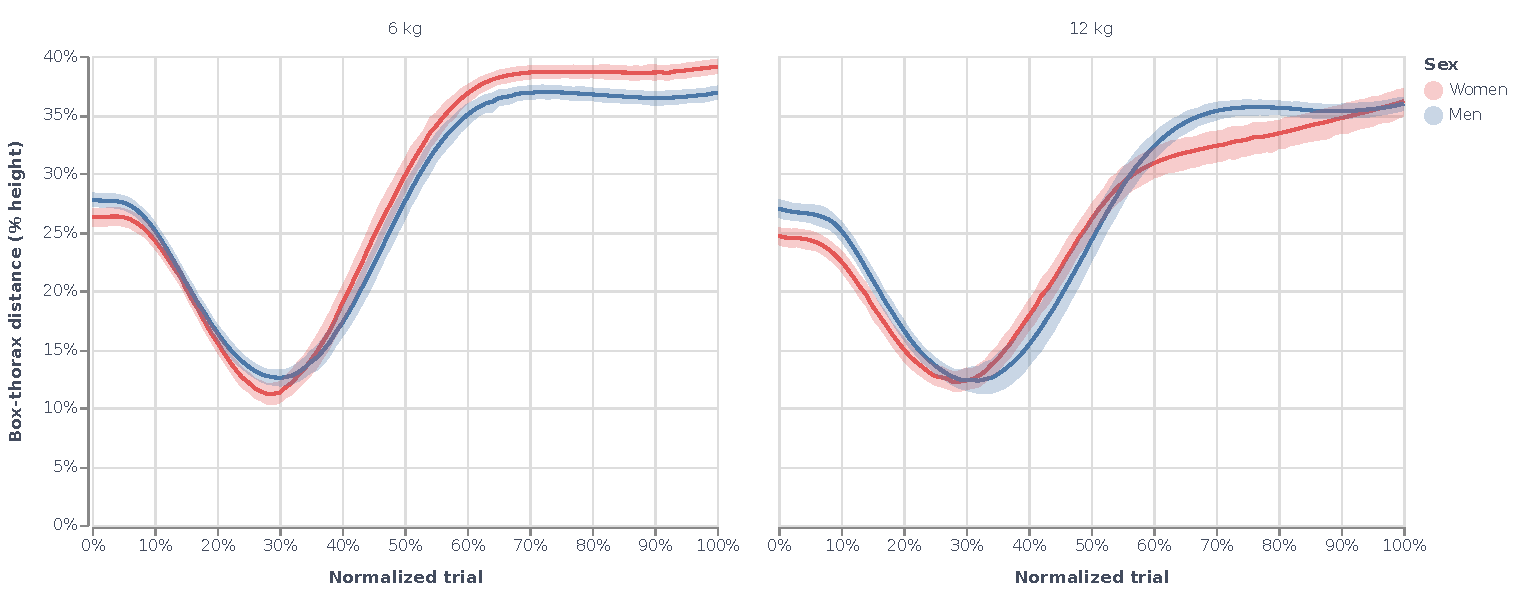
\includegraphics[width=1\linewidth]{fig/box-thorax.pdf}
    \caption{Mean (lines) and 95\% confidence interval (areas) of the box-thorax distance expressed in percentage of the participant's height by sex (women in red and men in blue) with a 6~kg (left panel) and 12~kg (right panel) box.}
\end{figure}

\begin{figure}[H]
    \centering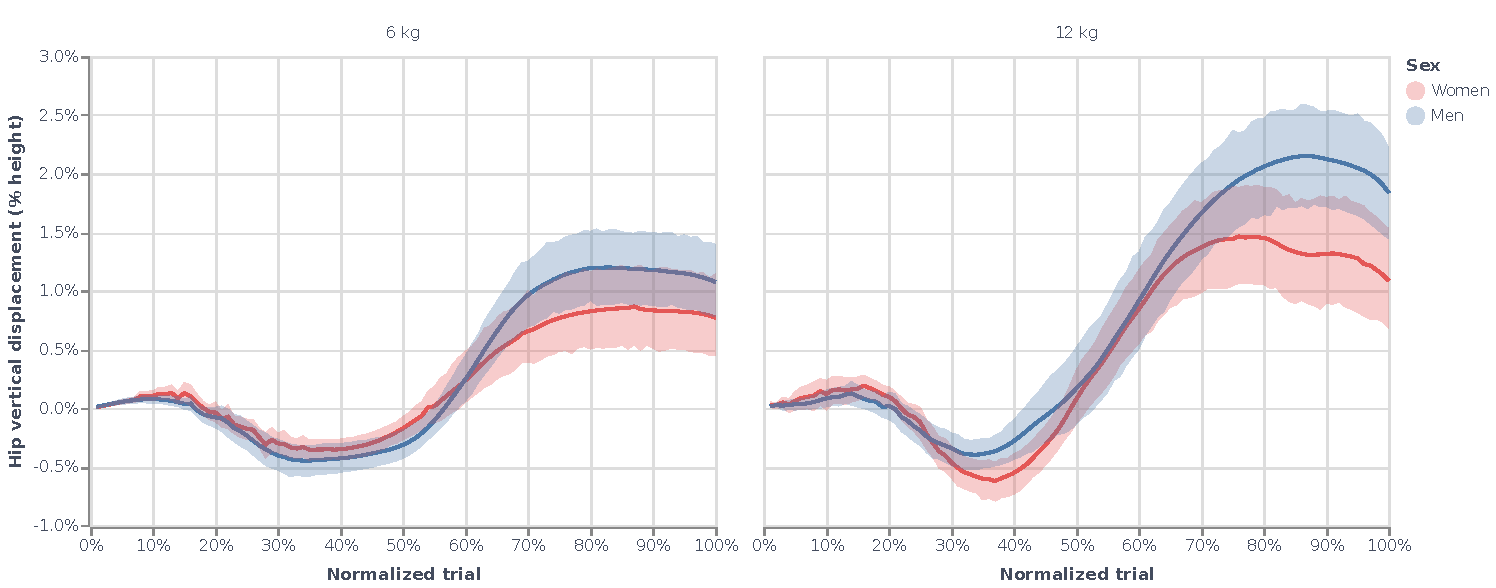
\includegraphics[width=1\linewidth]{fig/hip-displacement.pdf}
    \caption{Mean (lines) and 95\% confidence interval (areas) of the hip vertical displacement distance expressed in percentage of the participant's height by sex (women in red and men in blue) with a 6~kg (left panel) and 12~kg (right panel) box.}
\end{figure}

